\chapter{晶格振动和晶体的热学性质\label{ch:4}}

\noindent \textbf{1.\quad} 一维单原子晶格,在简谐近似下,考虑每一原子与其余所有原子都有作用,求格波的色散关系。

\noindent \textbf{解:}

设第 $n$ 个原子的势能函数为

\begin{equation*}
    U = \frac{1}{2} \sum_{\substack{m=-\infty\\(m \ne 0)}}^{\infty} \beta_m \left(x_n - x_{n+m}\right)^2
\end{equation*}

其中,$\beta_m$ 为与第 $n$ 个原子的相距 $ma$ 的原子间的恢复力常数,$a$ 为晶格常数。则第 $n$ 个原子的受力为

\begin{align*}
    F_n &= -\frac{\partial U}{\partial x_n} \\
    &= \sum_{\substack{m=-\infty\\(m \ne 0)}}^{\infty} \beta_m \left(x_{n+m} - x_n\right) \\
    &= \sum_{m=1}^{\infty} \left[\beta_m (x_{n+m}-x_n) + \beta_{-m} (x_{n-m}-x_n)\right] \\
    &= \sum_{m=1}^{\infty} \beta_m (x_{n+m}+x_{n-m}-2 x_n)
\end{align*}

其中,利用了 $\beta_m=\beta_{-m}$ 。第 $n$ 个原子的运动方程为

\begin{equation*}
    M \ddot{x}_n = F_n = \sum_{m=1}^{\infty} \beta_m (x_{n+m}+x_{n-m}-2 x_n)
\end{equation*}

令其试解为

\begin{equation*}
    x_n = A e^{i[qna-\omega t]}
\end{equation*}

代入运动方程,可得

\begin{align*}
    -M \omega^2 &= \sum_{m=1}^{\infty} \beta_m (e^{iqma} + e^{-iqma} - 2) \\
    &= \sum_{m=1}^{\infty} 2\beta_m [\cos(qma)-1] \\
    &= -\sum_{m=1}^{\infty} 4\beta_m \sin^2 \left(\frac{qma}{2}\right)
\end{align*}

因此

\begin{equation*}
    \omega^2 = \frac{1}{M} \sum_{m=1}^{\infty} 4\beta_m \sin^2 \left(\frac{qma}{2}\right)
\end{equation*}

\noindent \textbf{2.\quad} 聚乙烯链 $\cdots-CH=CH-CH=CH-\cdots$ 的伸张振动,可以采用一维双原子链模型来描述,原胞两原子质量均为 $M$, 但每个原子与左右的力常数分别为 $\beta_1$ 和 $\beta_2$,原子链的周期为 $a$。证明振动频率为

\begin{equation*}
    \omega_\pm^2 = \frac{\beta_1+\beta_2}{M} \left[1 \pm \left(1 - \frac{4\beta_1 \beta_2 \sin^2 \frac{qa}{2}}{(\beta_1+\beta_2)^2}\right)^{1/2}\right]
\end{equation*}

\noindent \textbf{解:}

单键及双键的长分别为 $b_1$ 和 $b_2$,而 $a=b_1+b_2$

原子 $(n, 1)$ 与 $(n, 2)$ 的运动方程分别为

\begin{align*}
    M \ddot{u}(n, 1) &= \beta_1 [u(n-1, 2)-u(n, 1)] - \beta_2 [u(n, 1)-u(n, 2)] \\
    M \ddot{u}(n, 2) &= \beta_2 [u(n, 1)-u(n, 2)] - \beta_1 [u(n, 2)-u(n+1, 1)]
\end{align*}

令这两个方程的试解为

\begin{align*}
    u(n, 1) &= A e^{i(qna-\omega t)} \\
    u(n, 2) &= B e^{i[q(na+b_2)-\omega t]}
\end{align*}

把试解代入运动方程得

\begin{align*}
    -M \omega^2 A &= \beta_1 [B e{-iq b_1} - A] - \beta_2 [A - B e^{iq b_2}] \\
    -M \omega^2 B &= \beta_2 [A e{-iq b_2} - B] - \beta_1 [B - A e^{iq b_1}]
\end{align*}

有非零解的条件为

\begin{equation*}
    \begin{vmatrix}
        \beta1 + \beta_2 - M \omega^2 & -\beta_1 e^{-iq b_1} - \beta e^{iq b_2} \\
        -\beta_2 e^{-iq b_2} - \beta_1 e^{iq b_1} & \beta_1 \beta_2 - M \omega^2
    \end{vmatrix} = 0
\end{equation*}

解得

\begin{equation*}
    (M \omega^2)^2 - 2(\beta_1+\beta_2) (M \omega^2) + (\beta_1+\beta+2)^2 - \left[\beta_1^2 + \beta_2^2 + 2\beta_1\beta_2 \cos q(b_1+b_2)\right] = 0
\end{equation*}

利用 $b_1+b_2=a$,方程的解为

\begin{equation*}
    \omega_\pm^2 = \frac{\beta_1+\beta_2}{M} \left[1 \pm \left(1 - \frac{4\beta_1 \beta_2 \sin^2 \frac{qa}{2}}{(\beta_1+\beta_2)^2}\right)^{1/2}\right]
\end{equation*}


\noindent \textbf{3.\quad} 求一维单原子链的振动模式密度 $g(\omega)$,若格波的色散可以忽略,其 $g(\omega)$ 具有什么形式,比较这两者的 $g(\omega)$ 曲线。

\noindent \textbf{解:}

(1) 一维单原子链的晶格振动的色散关系为

\begin{equation*}
    \omega = \omega_m \left| \sin\frac{qa}{2} \right|
\end{equation*}

其中

\begin{equation*}
    \omega_m = 2 \sqrt{\frac{\beta}{M}}
\end{equation*}

此函数为偶函数,只考虑 $q \ge 0$ 的情况,下式右边乘 $2$。$[\omega, \omega+\dif\omega]$ 区间振动模式数目为

\begin{equation*}
    g(\omega) \dif \omega = 2 \times \frac{L}{2\pi} \frac{1}{\nabla \omega} \dif\omega
\end{equation*}

其中在一维情形下,

\begin{equation*}
    \nabla \omega = \frac{\dif \omega}{\dif q} = \frac{a}{2} \omega_m \cos \frac{qa}{2} = \frac{a}{2} \left(\omega_m^2 - \omega^2\right)^{\frac{1}{2}}
\end{equation*}

故色散关系为

\begin{equation*}
    g(\omega) = \frac{2L}{2\pi} \left(\omega_m^2 - \omega^2\right)^{-\frac{1}{2}} = \frac{2N}{\pi} \left(\omega_m^2 - \omega^2\right)^{-\frac{1}{2}}
\end{equation*}

其中,$L$ 为单链总长,$a$ 为晶格常数,因此,$N$ 为原子个数。

(2) 若格波没有色散,既只有一个 $\omega_E$ (爱因斯坦模型)。而且振动模式密度函 $g(\omega)$ 数满足下面关系归

\begin{equation*}
    \int g(\omega) \dif\omega = N
\end{equation*}

故 $g(\omega)$ 为 $\delta$ 函数

\begin{equation*}
    g(\omega) \dif\omega = N \delta(\omega-\omega_E)
\end{equation*}

(1)(2) 色散关系的曲线图如下:

\begin{figure}[htbp]
    \centering
    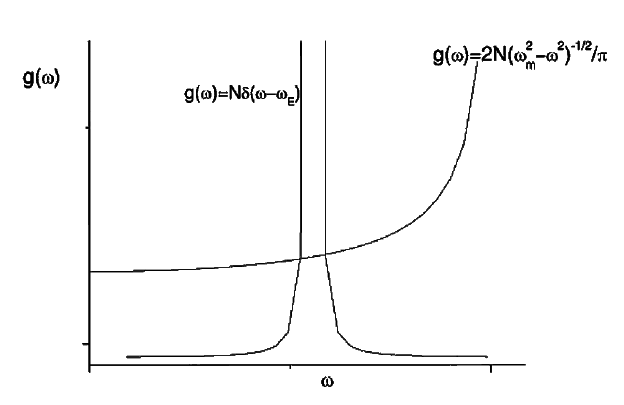
\includegraphics[width=0.5\textwidth]{pic/色散关系.png}
    \caption{色散关系}
    \label{fig:4.1}
\end{figure}

\noindent \textbf{4.\quad} 金刚石 (碳原子量为 $12$) 的杨氏模量为 \qty{e12}{N.m^{-2}},密度 $\rho=\qty{3.5}{g.cm^{-3}}$ 。试估算它的德拜温度 $\Theta_D=$?

\noindent \textbf{解:}

德拜温度为

\begin{equation*}
    \Theta_D = \frac{\hbar \omega_D}{k_B}
\end{equation*}

我们有

\begin{equation*}
    \omega_D = \left(\frac{6 \pi^2 N}{V}\right)^{\frac{1}{3}} V_s, \quad V_s = \sqrt{\frac{Y}{\rho}}
\end{equation*}

所以可得

\begin{align*}
    \Theta_D &= \frac{\hbar}{k_B} \sqrt{\frac{Y}{\rho}} \cdot \left(\frac{6 \pi^2 N}{V}\right)^{\frac{1}{3}} \\
    &= \frac{\hbar}{k_B} \sqrt{\frac{Y}{\rho}} \cdot \left(\frac{6 \pi^2 \rho}{M_C}\right)^{\frac{1}{3}} \\
    &= \frac{1.0546 \times 10^{-34}}{1.3807 \times 10^{-23}} \cdot \sqrt{\frac{10^{12}}{3.5 \times 10^3}} \left(\frac{6 \times 3.14^2 \times 3.5 \times 10^3}{12 \times 1.6605 \times 10^{-27}}\right)^{\frac{1}{3}} \unit{K} \\
    &\approx \qty{2817}{K} 
\end{align*}

\noindent \textbf{5.\quad} 试用德拜模型求晶体中各声频支格波的零点振动能。

\noindent \textbf{解:}

在德拜模型中,纵波与横波的最大振动频率均为 $\left(\frac{6 \pi^2 N}{V}\right)^{\frac{1}{3}} V_s$,其中 $\frac{1}{V_s^3}=\frac{1}{3} \left(\frac{1}{V_l^3}+\frac{2}{V_t^3}\right)$

\begin{equation*}
    g_l(\omega) = \frac{V}{2 \pi^2} \frac{\omega^2}{V_l^3}, \quad g_t(\omega) = \frac{V}{2 \pi^2} \frac{\omega^2}{V_t^3}
\end{equation*}

纵波的零点振动能为

\begin{align*}
    U_{0l} &= \int_0^{\omega_D} \frac{\hbar\omega}{2} \cdot g_l(\omega) \dif\omega \\
    &= \int_0^{\omega_D} \frac{\hbar\omega}{2} \cdot \frac{V}{2\pi^2} \frac{\omega^2}{V_l^3} \dif\omega \\
    &= \frac{\hbar V}{16 \pi^2 V_l^3} \omega_D^4
\end{align*}

同理可得,两支横波的零点振动能均为

\begin{align*}
    U_{0t} &= \int_0^{\omega_D} \frac{\hbar\omega}{2} \cdot g_t(\omega) \dif\omega \\
    &= \int_0^{\omega_D} \frac{\hbar\omega}{2} \cdot \frac{V}{2\pi^2} \frac{\omega^2}{V_t^3} \dif\omega \\
    &= \frac{\hbar V}{16 \pi^2 V_t^3} \omega_D^4
\end{align*}

故,总的零点振动能为

\begin{align*}
    U_0 &= U_{0l} + 2 U_{0t} \\
    &= \frac{\hbar V}{16 \pi^2 V_l^3} \omega_D^4 + 2 \frac{\hbar V}{16 \pi^2 V_t^3} \omega_D^4 \\
    &= \frac{3\hbar V}{16 \pi^2} \cdot \frac{1}{3} \left(\frac{1}{V_l^3}+\frac{2}{V_l^3}\right) \cdot \frac{6\pi^2 N}{V} V_s^3 \cdot \omega_D \\
    &= \frac{9N}{8} \hbar \omega_D
\end{align*}

\noindent \textbf{6.\quad} 一根直径为 \qty{3}{mm} 的人造蓝宝石晶体的热导率,在 \qty{30}{K} 的温度达到一个锐的极大值,试估计此极大值。(蓝宝石在 $T \ll \Theta_D = \qty{1000}{K}$ 时,$c_V=10^{-1} T^3 \unit{J.m^{-3}.K^{-1}}$)

\noindent \textbf{解:}

在低温情况下,热导率的表达式为

\begin{equation*}
    \kappa = \frac{1}{3} c_V v l
\end{equation*}

其中,$c_V=10^{-1} T^3 \unit{J.m^{-3}.K^{-1}}$, 而且由于直径很小,自由程 $l\approx d=\qty{3}{mm}$,所以

\begin{equation*}
    \kappa = 2.7 v
\end{equation*}

而声速 $v$ 由德拜模型求取,在德拜模型中,($N$为原胞个数)

\begin{equation*}
    \omega_D = \left(\frac{30\pi^2 N}{V}\right)^{\frac{1}{3}} V_s = \left(\frac{30 \pi^2 N \cdot M_{\ce{Al2O3}}}{V \cdot M_{\ce{Al2O3}}}\right)^{\frac{1}{3}} V_s, \quad \omega_D = \frac{\Theta_D k_B}{\hbar}
\end{equation*}

故,

\begin{equation*}
    V_s = \frac{\Theta_D k_s}{\hbar} \left(\frac{30 \pi^2 \rho}{M_{\ce{Al2O3}}}\right)^{-\frac{1}{3}} \approx \qty{6.84e3}{m.s^{-1}}
\end{equation*}

其中 $\rho=\qty{4}{g.cm^{-3}}$。

\begin{equation*}
    v = V_s \approx \qty{6.84e3}{m.s^{-1}}
\end{equation*}

代入 $\kappa=2.7 v$ 中,可得

\begin{equation*}
    \kappa = \qty{1.85e4}{W.m^{-1}.K^{-1}}
\end{equation*}

\noindent \textbf{7.\quad} \ce{Na} 和 \ce{Cl} 的原子量分别为 $23$ 和 $37$。氯化钠立方晶胞边长为 \qty{0.56}{nm},在 $[100]$ 方向可以看作是一组平行的离子链。离子间距 $d=\qty{0.28}{nm}$。\ce{NaCl} 晶体的杨氏模量为 \qty{5e10}{N.m^{-2}} 气如果全放射的光频率与 $q=0$ 的光频模频率相等,求对应的光波波长 (实验值为 \qty{61}{um}) 。

\noindent \textbf{解:}

在一维双原子链模型中,$q=0$ 时,光频模频率为

\begin{equation*}
    \omega(0) = \left[2\beta \left(\frac{1}{M_1}+\frac{1}{M_2}\right) \right]^{\frac{1}{2}}
\end{equation*}

杨氏模量为

\begin{equation*}
    Y = \frac{L}{A} \left(\frac{\partial F}{\partial l}\right)_T = \frac{d}{d^2} \beta
\end{equation*}

所以

\begin{equation*}
    \beta = dY
\end{equation*}

光波波长为

\begin{align*}
    \lambda &= cT = c \cdot \frac{2\pi}{\omega} \\
    &= \frac{2\pi c}{\left[2\beta \left(\frac{1}{M_1}+\frac{1}{M_2}\right)\right]^{\frac{1}{2}}} \\
    &= \frac{2\pi c}{\left[2dY \left(\frac{1}{M_1}+\frac{1}{M_2}\right)\right]^{\frac{1}{2}}} \\
    &\approx \qty{54.6}{um}
\end{align*}

\noindent \textbf{8.\quad} 立方晶体有三个弹性模量 $C_{11}, C_{12}$ 和 $C_{44}$。铝的 $C_{11}=\qty{10.82e10}{N.m^{-2}}, C_{44}=\qty{2.85e10}{N.m^{-2}}$,铝沿 $[100]$ 方向传播的弹性纵波的速度 $v_l=\sqrt{\frac{C_{11}}{\rho}}$,横波速度 $v_t=\sqrt{\frac{C_{44}}{\rho}}$,\ce{Al} 的密度 $\rho=\qty{2.70e3}{kg.m^{-3}}$ 气求德拜模型中铝的振动模式密度 $g(m)$。

\noindent \textbf{解:}

德拜模型中,振动模式密度为

\begin{equation*}
    g(\omega) = \frac{3V}{2\pi^2} \frac{\omega^2}{V_s^3}, \quad (\omega \le \omega_D)
\end{equation*}

其中

\begin{equation*}
    \omega_D = \left(\frac{6\pi^2 N}{V}\right)^{\frac{1}{3}} V_s, \quad \frac{1}{V_s^3} = \frac{1}{3} \left(\frac{1}{V_l^3}+\frac{2}{V_t^3}\right)
\end{equation*}

将 $v_l=\sqrt{\frac{C_{11}}{\rho}}, v_t=\sqrt{\frac{C_{44}}{\rho}}$ 代入上式可得

\begin{align*}
    \frac{1}{V_s^3} &= \frac{1}{3} \left(\frac{1}{V_l^3}+\frac{2}{V_t^3}\right) \\
    &= \frac{1}{3} \left[\left(\frac{\rho}{C_{11}}\right)^{\frac{3}{2}}+2\left(\frac{\rho}{C_{44}}\right)^{\frac{3}{2}}\right] \\
    &\approx \qty{2.075e-11}{m^{-3}.s^3}
\end{align*}

所以

\begin{equation*}
    V_s = \qty{3.64e3}{m·s^{-1}}
\end{equation*}

代入 $\omega_D$ 中,

\begin{align*}
    \omega_D &= \left(\frac{6\pi^2 N}{V}\right)^{\frac{1}{3}} V_s \\
    &= \left(\frac{6\pi^2 N \cdot M_{\ce{Al}}}{V \cdot M_{\ce{Al}}}\right)^{\frac{1}{3}} V_s \\
    &= \left(\frac{6\pi^2 \rho}{M_{\ce{Al}}}\right)^{\frac{1}{3}} V_s \\
    &\approx \qty{5.56e13}{rad.s^{-1}}
\end{align*}

所以

\begin{align*}
    g(\omega) &= \frac{3V}{2\pi^2} \frac{\omega^2}{V_s^3} \\
    &= \frac{3}{2 \times 3014^2} \times 2.075 \times 10^{-12} \omega^2 V \\
    &\approx 3.157 \times 10^{-12} \omega^2 V
\end{align*}

其中

\begin{equation*}
    \omega \le \omega_D = \qty{5.56e13}{rad.s^{-1}}
\end{equation*}
